\chapter{Implementatie van een \glsentrytext{GPG} Web Of Trust}
\label{ch:implementatie-van-een-gpg-web-of-trust}

Dit hoofdstuk behandelt hoe een \gls{GPG} Web Of Trust kan worden
geïmplementeerd in
een bedrijf. Onder andere wordt de configuratie van \gls{GPG} onderzocht en
de beste
instellingen geconcludeerd.

\section{Gebruikte algoritmes}
\label{sec:gebruikte-algoritmes}

\gls{GPG} gebruikt meerdere algoritmes om de publieke/private encryptie en
digitale
handtekeningen toe te passen. Het kiezen van het juiste algoritme en de
configuratie hiervan heeft een impact op veiligheid van de sleutels en de
compatibiliteit met andere systemen. We vergelijken de belangrijkste algoritmes
in \gls{GPG}. Het meest gebruikte algoritme is RSA gevolgd door DSA. ECC, wat
staat
voor Elliptic Curve Cryptography, is een nieuwer algoritme dat nog aan
populariteit moet winnen.

RSA is een veelgebruikt asymmetrische crypto en ontleent zijn naam aan zijn
auteurs, zijnde Rivest, Shamir en Adleman. Het gebruik van RSA nam vooral toe
naar het verlopen van het patent in de Verenigde Staten.

DSA, wat staat voor Digital Signature Algorithm, is een variant op het ElGamal
handtekening schema dat ontwikkeld is door de NSA. Het wordt veel gebruikt en
vind het grootste deel van zijn toepassing in oudere toepassingen. DSA vereist
absolute zekerheid van de geheimhouding, willekeurigheid en uniciteit van een
willekeurige waarde. Indien enkele bits van de willekeurige waarde gelekt
werden, kon de private sleutel bepaald worden. Dit bleek uiterst gevaarlijk toen
de NSA een met opzet gebrekkige random number generator publiceerde genaamd
Dual\_EC\_DRBG \autocite{Perlroth2013NsaRng, Zetter2013NsaRng, GuardianNsaRng}.
Het bedrijf genaamd RSA Security, niet te verwarren met het algoritme, dat een
zeer invloedrijke firma is qua computer beveiliging heeft na een betaling van 10
miljoen US-dollar door de NSA, Dual\_EC\_DRBG de standaard gemaakt in zijn
programma, BSafe. Zo werd een beveiligingsbedrijf dat bekend stond om zijn
strijd voor privacy en security de grootste verspreider van deze backdoor
\autocite{Menn2013NsaRsa}.

ECC is nieuwere vorm van public/private key encryption. Het heeft als voordeel
dat de sleutel kleiner is en dat in vergelijking met RSA, kleinere modulus
sleutels nodig zijn om dezelfde veiligheid te bekomen. Een 256 bit ECC-sleutel
staat ongeveer gelijk qua veiligheid aan een 3072 bit RSA-sleutel. Ook is het
aanmaken en verifiëren van digitale handtekeningen sneller.
\autocite{HighSpeedHighSecuritySignatures} Dit is vooral handig op systemen met
een zwakkere processoren zoals Internet Of Things apparaten. Het nadeel van de
implementaties van ECC zoals ECDSA (Elliptic Curve Digital Signature Algorithm)
en Curve 25519 is dat ze nog niet wijdverspreid of nog niet gestandaardiseerd
zijn. Dit zorgt ervoor dat compatibiliteit met andere systemen niet zeker is.

We kunnen concluderen dat tot ECC-implementaties verder uitgewerkt en
gestandaardiseerd zijn, het best is om RSA te gebruiken.

\section{RSA-sleutel bit grootte}
\label{sec:rsa-sleutel-bit-grootte}

De bit grootte van een RSA-sleutel was 512 bits vanaf 1974 tot in de jaren 80.
In de latere jaren 90 werd de aanbevolen grootte verhoogt naar 768 voor
gebruikers en 1024 voor bedrijven \autocite{OriginalRSAKeySizeRecommendations}.
In 2015 publiceerde het \acrshort{NIST} SP 800-57 dat 2048 aanraadt voor
individuen en
apparaten. De grootte van 2048 tot 3072 wordt aangeraden voor, onder andere,
certificaat autoriteiten
\autocite{NISTKeyManagementRecommendationApplicationSpecific}. De 3072 bit
versie wordt aangeraden indien er geen problemen zijn met interoperabiliteit met
andere apparaten. RSA-768 is de grootste modulo die ooit is gefactoriseerd en
publiek bekend is gemaakt \autocite{FactorizationOf768BitRSA}. Dit proces nam
vier jaar in beslag. \textcite{FactorizationOf768BitRSA} voorspeld dat het
factoriseren van een 1024 bit RSA-modulus binnen het bereik ligt van academische
inspanning.

RSA 2048 zou moeten volstaan tot 2030
\autocite{NISTKeyManagementRecommendationGeneral, NISTAlgorithmesAndKeyLengths}.
Hiermee wordt bedoeld dat het technisch niet haalbaar is om een RSA 2048 bit
sleutel te raden. GitHub raad 4096 bits aan
\autocite{GithubGeneratingANewGPGKey}. Het verdubbelen van RSA-bit grootte heeft
echter niet een verdubbeling van de beveiliging tot gevolg. Een RSA 2048 sleutel
geeft 112 bits beveiliging en RSA 2048 geeft ongeveer 140 bits aan beveiliging.
Het verdubbelen van de grootte van de sleutel heeft in vergelijking weinig
invloed op de toegevoegde beveiliging \autocite{GnuPGFAQ}. Een bit grootte boven
2048 wordt dan ook enkel aangeraden als de bijkomende vertraging niet kritiek is
voor de toepassing. Een voorbeeld van een toepassing waar snelheid kritiek is,
is bijvoorbeeld een webservice of website.

\begin{lstlisting}[language=bash, caption={Commando om de snelheid van RSA te
testen}]
$ openssl speed rsa
\end{lstlisting}

Het resultaat van dit commando kan gevonden worden in tabel
\ref{tab:rsa-speed-test}.

\begin{table}[H]
	\centering
	\begin{tabular}{ l | l | l | r | r }
		& \multicolumn{1}{c}{sign} & \multicolumn{1}{c}{verify} &
		\multicolumn{1}{c}{sign/s} & \multicolumn{1}{c}{verify/s} \\
		\hline
		rsa  512 bits & 0.000048s & 0.000004s &  20841.1 & 274224.6 \\
		rsa 1024 bits & 0.000137s & 0.000009s &   7304.4 & 110915.7 \\
		rsa 2048 bits & 0.000624s & 0.000028s &   1603.2 &  36341.9 \\
		rsa 4096 bits & 0.006696s & 0.000100s &    149.3 &   9974.3 \\
	\end{tabular}
	\caption{Snelheid van RSA getest in Ubuntu 16.04, i7-4700HQ (3.4 GHz), 12 GB
		DDR3 1600 MHz RAM}
	\label{tab:rsa-speed-test}
\end{table}

Tabel \ref{tab:rsa-speed-test} kan weergegeven als box plot zoals in grafiek
\ref{fig:rsa-sign-verify-speed-graph}.

\begin{figure}[H]
	\centering
	\begin{tikzpicture}
	\begin{axis}[
		x tick label style={/pgf/number format/1000 sep=},
		ylabel = Aantal milliseconden per bewerking (ms),
		enlargelimits = 0.02,
		legend style={at={(0.5, -0.05)}, anchor=north, legend columns=-1},
		ybar interval=0.8,
		width = \textwidth,
		height = .90\textheight,
		symbolic x coords = {512,1024,2048,4096,8192},
	]
		\addplot
		coordinates {(512, 0.048) (1024, 0.137)
			(2048, 0.624) (4096, 6.696) (8192, 0)};
		\addplot
		coordinates {(512, 0.004) (1024, 0.009)
			(2048, 0.028) (4096, 0.10) (8192, 0)};
		\legend{Sign, Verify}
	\end{axis}
	\end{tikzpicture}
	\caption{Weergave van het aantal milliseconden per ondertekening en
		verificatie
		voor de verschillende bit groottes}
	\label{fig:rsa-sign-verify-speed-graph}
\end{figure}

We kunnen concluderen dat de toegevoegde veiligheid van 4096 bit sleutels in
vergelijking met 2048 bit sleutels niet opweegt tegen het enorme
snelheidsverlies.

\section{Distributie van sleutels}
\label{sec:distributie-van-sleutels}

De distributie van persoonlijke sleutels is een zeer belangrijk aspect van de
veilige werking van het proces. Niemand behalve de eigenaar van de sleutel mag
de sleutel en bijhorende wachtwoord bezitten en enkel het bedrijf mag sleutels
aanduiden als vertrouwd. Ook mag het niet mogelijk zijn om de private sleutel te
onderscheppen met een \textit{Man In The Middle attack}.

In een Web Of Trust is het zo dat elke persoon verantwoordelijk is voor het
identificeren en ondertekenen van de personen met wie hij zal communiceren. Om
te zorgen dat elke nieuwe werknemer niet moet persoonlijk zich identificeren met
elke andere werknemer zou het best zijn als er de mogelijkheid om deze centraal
te kunnen valideren. Het is mogelijk om één centrale sleutel compleet te
vertrouwen of om meerdere centrale sleutels marginaal te vertrouwen. In dit
voorbeeld zullen we één centrale sleutel hebben.

\subsection{De centrale sleutel(s)}
De centrale sleutel vervult de rol van centrale autoriteit. De private centrale
sleutel, O\textsubscript{priv}, wordt beheerd door een medewerker die het volste
vertrouwen van de organisatie geniet. De publieke sleutel is voor iedereen
beschikbaar. Dit kan op verschillende manieren.

Indien alle werkstations onder toezicht van het interne IT departement vallen,
dan kan de publieke sleutel gemakkelijk voorgeïnstalleerd zijn op het
werkstation. Toegang van thuis uit naar de centrale sleutel is niet mogelijk op
deze manier ook als een medewerker zijn of haar eigen toestel gebruikt zal deze
methode tekort komen. Daarom zou het gemakkelijker zijn indien op de website van
het bedrijf, de sleutel beschikbaar is. Deze website zou dan wel moeten
uitgerust zijn met een HTTPS certificaat zodat het niet mogelijk is om deze aan
te passen met een MITM aanval.

\subsection{Bij aankomst van een nieuwe werknemer}
\label{subsec:aankomst-nieuwe-werknemer}
In dit voorbeeld zal Tim, een nieuwe medewerker, geïntroduceerd worden in het
Web Of Trust. Hiervoor worden volgende stappen ondernomen.

\begin{itemize}
	\item Genereren van een eigen sleutelpaar
	\item Centrale publieke sleutel ondertekenen
	\item Centrale sleutel(s) aanduiden als designated revoker
	\item Eigen publieke sleutel verzenden naar de keyserver
	\item Het nieuwe sleutelpaar wordt ondertekend door de centrale sleutel
\end{itemize}

Tim genereert een nieuw sleutelpaar beveiligd met een zelfgekozen, sterk
wachtwoord (zie \fullref{sec:wachtwoordsterkte}). Dit wordt best gedaan via een
programma dat bepaalde eigenschappen zoals bit sterkte en het gebruikte
algoritme, RSA of DSA, afdwingt om zo de soorten sleutels die in het bedrijf
gebruikt worden consistent te houden. Dit zou eventuele problemen met mogelijke
migraties van sleutels naar ID-cards vermijden alsook het verminderen van bugs
in het verwerken van de sleutels met software. Deze software zou namelijk kunnen
verwachten dat de sleutel een RSA sleutel is of geen DSA ondersteunen.
Consistentie is belangrijk.

De sleutel moet natuurlijk ergens worden opgeslagen. Indien de medewerker maar
één werkstation gebruikt, kan de sleutel hierop blijven. Dit is echter bij de
meeste bedrijven niet het geval. Denk maar aan thuiswerk en het gebruik van
smartphones.

Een veelgebruikt medium, namelijk een USB-apparaat, kan hiervoor gebruikt
worden. Om de private sleutel zo veilig mogelijk te bewaren encrypteren we deze
best. Er komt dus nog een laag encryptie bij. Het USB-apparaat kan
gepartitioneerd worden om zowel een geëncrypteerd deel als een niet
geëncrypteerd deel te bevatten. Dit kan handig zijn om publieke sleutels bij te
houden zodat deze gemakkelijk te exporteren zijn en kan dienen om de eigenaar
van de USB te identificeren terwijl de private sleutel veilig bewaard wordt. Dit
wordt aangetoond in figuur \ref{fig:usb-device}.

\begin{figure}[H]
	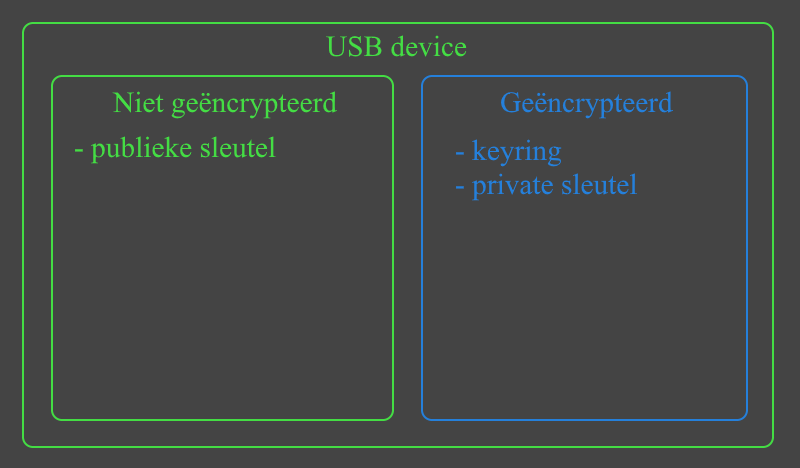
\includegraphics[width=\textwidth,keepaspectratio]{img/usb-store-with-gpg-keys.png}
	\centering
	\caption{USB apparaat waarop de private en publieke sleutel wordt bewaart.}
	\label{fig:usb-device}
\end{figure}

Tim zijn sleutel moet nog gevalideerd worden door de centrale sleutel en vice
versa. De publieke centrale sleutel wordt nu geïmporteerd op het werkstation van
Tim. Deze zou ook voorgeïnstalleerd kunnen staan  Dit kan via meerdere manieren,
keyservers, USB, … Hierna moet de fingerprint van de sleutel vergeleken en
gevalideerd worden. Nadat dit gebeurd is, ondertekent Tim de publieke centrale
sleutel met zijn sleutel en geeft deze het juiste vertrouwensniveau. Dit zal in
het algemeen marginal of full zijn, afhankelijk van het feit of er meerdere of
één centrale sleutel is. Tim duid de centrale sleutel ook aan als designated
revoker. Hierdoor kan het bedrijf de sleutel terugtrekken indien nodig. Het
proces dat zojuist werd beschreven waarin Tim de centrale sleutel(s) importeert,
kan automatisch gedaan worden door een intern programma dat vooraf
geïnstallleerd was op het werkstation.

De publieke sleutel van Tim moet nu nog geïmporteerd worden in het netwerk van
het bedrijf en ondertekend worden door de centrale sleutel. Dit is nodig omdat
anders andere medewerkers de sleutel van Tim niet zullen vertrouwen. Tim, of het
programma dat de sleutels van de nieuwe medewerkers aanmaakt, geeft hiervoor de
publieke sleutel door aan de beheerder(s) van het centrale netwerk. Hierna
bevestigen Tim en de beheerder(s) van de centrale sleutel dat de fingerprint van
de sleutel overeenkomt. Bij succesvolle vergelijking wordt Tim zijn sleutel
ondertekend door de centrale sleutel en daarna geëxporteerd naar de private
keyserver van het bedrijf. Tim importeert zijn publieke sleutel van de private
keyserver zodat hij de ondertekening van zijn sleutel door de centrale
sleutel(s) lokaal heeft. Nu kan Tim aan het werk. Iedereen die een digitale
handtekening tegenkomt van Tim of wilt communiceren met Tim zal zien dan zijn
sleutel wordt vertrouwd.

Alhoewel Tim aan het werk kan moet er nog een probleem opgelost worden. De
private sleutel bestaat namelijk maar op één plaats. Indien deze verloren raakt,
zal Tim alle data die ooit met zijn publieke sleutel is geëncrypteerd, voor
altijd kwijt zijn. Het is daarom een goed idee om twee USB-apparaten te maken.

\subsection{Online opslag van de private sleutel}
\label{subsec:online-opslag-van-de-private-sleutel}

Het is niet handig om het opslagapparaat overal naartoe mee te nemen. Het
aansluiten met smartphones kan ook een probleem worden indien er geen poort
aanwezig is om het apparaat op aan te sluiten. Om dit op te lossen zou het
mogelijk kunnen zijn om de private sleutel online op te slaan (i.e. cloud) en
deze dan te downloaden wanneer nodig. Er zijn echter bepaalde maatregelen nodig
om zeker te kunnen zijn dat niemand behalve de bezitter van de sleutel, toegang
heeft tot de private sleutel.

De cloud omgeving waarop deze private sleutel wordt opgeslagen moet \textit{zero
knowledge} zijn. Hiermee wordt bedoeld dat de provider van de cloud omgeving
niet in staat mag zijn om de inhoud van de container te lezen. De container in
dit geval is soort map waarin alle geëncrypteerde bestanden zitten. Ook mag een
\textit{Man In The Middle attack} niet resulteren in een gecompromitteerde
private sleutel.

De container mag enkel op het eigen apparaat gedecrypteerd worden. Het
wachtwoord voor decryptie mag het eigen apparaat niet verlaten. Dit voorkomt dat
private sleutel kan bekeken worden door het onderscheppen van de gedecrypteerde
container of het onderscheppen van het wachtwoord. Figuur
\ref{fig:online-zero-knowledge-container} legt uit hoe zo’n systeem kan werken.

\begin{figure}[H]
	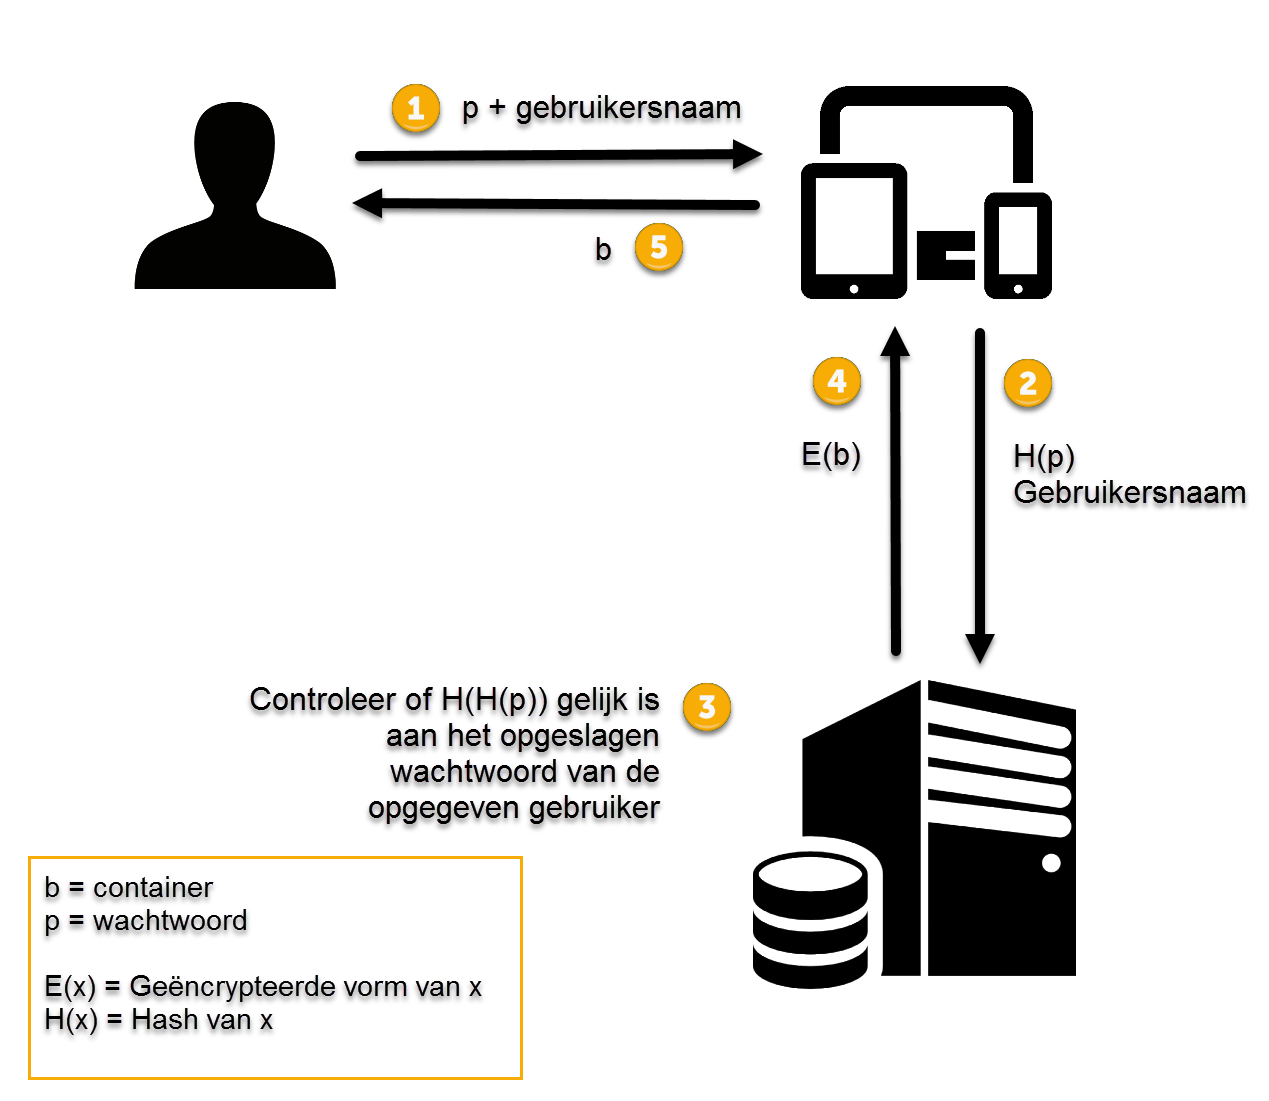
\includegraphics[width=\textwidth,keepaspectratio]{img/encrypted-container-sharing.png}
	\centering
	\caption{Een zero knowledge structuur}
	\label{fig:online-zero-knowledge-container}
\end{figure}

Met deze implementatie verlaat het wachtwoord van de gebruiker, en dus ook het
wachtwoord van de container, het apparaat van de gebruiker niet. Het is sowieso
niet mogelijk om de container te decrypteren zonder het wachtwoord en het
wachtwoord kan niet onderschept worden door een \textit{Man In The Middle
	attack}.

Indien de database met alle gebruikersnamen en wachtwoorden wordt
gecompromitteerd kan een aanvaller nog altijd niet de geëncrypteerde container
buitmaken omdat tijdens de aanmeldpoging het wachtwoord nog eens
\glslink{hash}{gehasht} wordt.
De database bevat namelijk \textit{H(H(p))} en als \textit{H(H(p))} wordt
ingegeven tijdens een aanmelding zal de vergelijking
\textit{H(H(H(p)))~=~H(H(p))} worden. Dit zal natuurlijk een foutieve
aanmeldingspoging tot gevolg
hebben.

Een dienst zoals dit opzetten vereist een grote kennis van zowel encryptie als
netwerking. Het is daarom niet aangeraden om een dienst zoals dit zelf te maken
zonder de nodige know-how. Er zijn commerciële bedrijven die zo’n dienst
aanbieden, een voorbeeld hiervan is SpiderOak.

\section{Wachtwoordsterkte}
\label{sec:wachtwoordsterkte}

Een belangrijk onderdeel van de sterkte van de encryptie van het opslagapparaat
alsook de sterke van de sleutel is de sterkte van de gekozen wachtwoorden. We
hebben twee wachtwoorden op dit moment, het wachtwoord dat het opslagapparaat
beveiligt en het wachtwoord dat de private sleutel zelf beveiligt. Beide moeten
sterk genoeg zijn om alle soorten van \textit{bruteforce} aanvallen niet
haalbaar te maken.

\begin{figure}[H]
	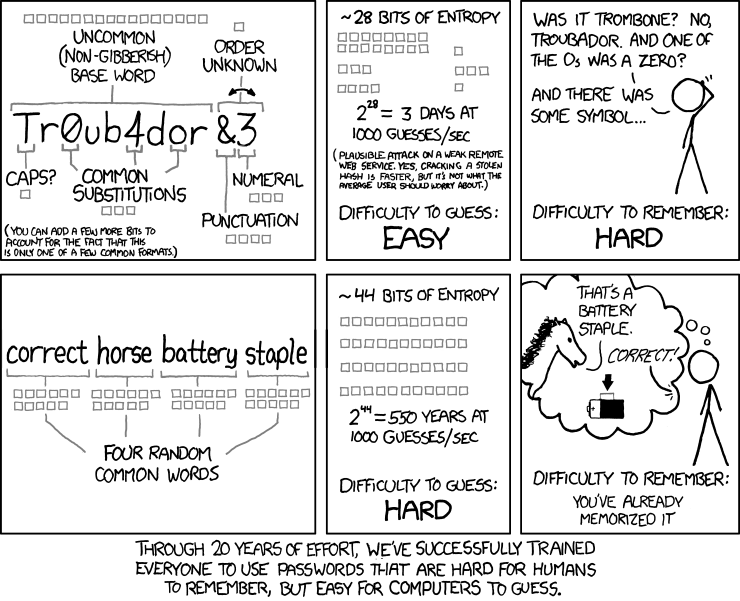
\includegraphics[width=\textwidth,keepaspectratio]{img/password-strength-xkcd.png}
	\centering
	\caption{XKCD: \url{https://xkcd.com/936/}}
	\label{fig:wachtwoord-sterkte-xkcd}
\end{figure}

Figuur \ref{fig:wachtwoord-sterkte-xkcd} toont een bekende XKCD-comic over
wachtwoord sterkte en de wachtwoord vereisten die vaak gevraagd worden.

Uit een voorstel voor een publicatie (zie
\textcite{NISTDigitalIdentityGuidelines}) dat het \acrlong{NIST}, kortweg
\acrshort{NIST}, gepubliceerd heeft betreffende
wachtwoorden en best practices kunnen we enkele zaken concluderen. Wachtwoorden
moeten minstens 8 karakters lang zijn, dit minimum mag verhoogd worden indien
het gaat over gevoelige informatie. Het wachtwoord van de geëncrypteerde
container alsook het wachtwoord van de private sleutel valt hieronder. Een
minimumlengte van 16 karakters moet verplicht worden. Een nog langer wachtwoord
is aangeraden. Wachtwoordzinnen zijn een goede oplossing voor het onthouden van
langere wachtwoorden zoals de XKCD comic (figuur
\ref{fig:wachtwoord-sterkte-xkcd}) ook aangeeft.

Het \acrshort{NIST} zegt verder dat het laten vervallen van wachtwoorden is
afgeraden
aangezien dit de gebruiker niet ten goede komt en kan leiden tot een niet
veilige manier voor het onthouden van het wachtwoord. Een voorbeeld van wat er
kan gebeuren in dit geval is wat er gebeurd is met het Franse tv-kanaal
TV5Monde. In een uitzending werd gefilmd bij een medewerker zijn burea. Op de
muur erachter hingen echter verscheidene notities waaronder wachtwoorden en
gebruikersnaam combinaties \autocite{MachkovechMonde}. Wachtwoorden mogen enkel
vervallen wanneer ze gecompromitteerd zijn.

Wachtwoord tips zijn ten zeerste afgeraden sinds ze teveel kunnen helpen met het
raden van het wachtwoord door aanvallers. Dit gebeurde na de hack van Adobe
waarna 150 miljoen wachtwoorden, gebruikersnamen, en wachtwoordhints werden
buitgemaakt en online gezet. De wachtwoordhints waren zo specifiek dat, door een
combinatie met een slechte \gls{hash}/encryptie methode, een grote hoeveelheid
van de
wachtwoorden herleidbaar was \autocite{HernGuardianAdobeLeak}.

Wachtwoord hergebruik is niet afdwingbaar maar moet sterk afgeraden worden.
Indien hetzelfde wachtwoord gebruikt wordt voor de geëncrypteerde container en
de private sleutel, wordt de veiligheid gehalveerd. Indien een van de
wachtwoorden wordt gebruikt voor een andere service is de veiligheid van het
wachtwoord enkel afhankelijk van de manier waarop deze service met het
wachtwoord omgaat.

\section{Verlies wachtwoord of private sleutel}
\label{sec:verlies-wachtwoord-of-private-sleutel}
Wanneer de mogelijkheid bestaat dat een wachtwoord van een private sleutel
gecompromitteerd is, maar de private sleutel zelf niet, dan moet de eigenaar van
de sleutel een nieuw wachtwoord instellen voor de sleutel. Deze wijziging heeft
enkel effect op de private sleutel. Hierdoor is propagatie in het Web Of Trust
niet nodig.

Indien het wachtwoord van een private sleutel verloren is gegaan, met andere
woorden, de eigenaar van de sleutel is zijn wachtwoord vergeten, of de private
sleutel zelf is mogelijks gecompromitteerd, dan moet de sleutel teruggetrokken
worden. Dit voorkomt dat er misbruik kan gemaakt worden van de sleutel. De
volgende stappen dienen ondernomen te worden. De designated revoker van de
gecompromitteerde sleutel moet zo snel mogelijk op de hoogte gebracht worden. De
designated revoker genereert direct een revocation certificate voor de
gecompromitteerde sleutel. Hierna exporteert de designated revoker dit
revocation certificate naar de keyserver. De \gls{GPG} client die op elk
werkstation
van de werknemers staat, zal tijdens het automatisch verversen van sleutels, het
revocation certificaat binnenhalen. Op deze manier wordt de terugtrekking
doorheen het netwerk gepropageerd.

Afhankelijk van hoe groot de kans is geweest op misbruik, moet gecontroleerd
worden of dit ook het geval geweest is. Dit benadrukt opnieuw het feit dat het
belangrijk is om zo snel mogelijk te reageren om de kans op, onder andere, een
ongewenste handtekening zo klein mogelijk te maken.

Om de werknemer verder te kunnen laten werken moeten de stappen van een nieuwe
werknemer opnieuw uitgevoerd worden (zie subsectie
\fullref{subsec:aankomst-nieuwe-werknemer}). Hetzelfde opslagapparaat kan
gebruikt worden nadat de geëncrypteerde partitie verwijderd is.

\section{Verlies van de geëncrypteerde container}
\label{sec:verlies-geencrypteerde-container}

Het verlies van de geëncrypteerde container is niet ideaal maar betekent niet
dat de private sleutel gecompromitteerd is. Als het wachtwoord van de container
of het wachtwoord van de private sleutel de wachtwoordsterkte vereisten volgt,
dan is het goed mogelijk dat een aanvaller met alle computerkracht in de wereld
er niet in slaagt om het wachtwoord te achterhalen.

Indien er een backup is van de private sleutel dan is het niet nodig om het
sleutelpaar terug te trekken. We vertrouwen immers op de twee lagen encryptie
die ervoor moeten zorgen dat de sleutel niet kan gebruikt worden om e-mails, die
gestuurd zijn naar de betreffende medewerker, te decrypteren. Indien er geen
back-up is zal de designated revoker het sleutelpaar terugtrekken en zal het
proces voor een nieuw sleutelpaar doorlopen worden.
